\documentclass{article}
\usepackage{graphicx}
\usepackage[a4paper, left=2cm, right=2cm, top=2.5cm, bottom=2cm]{geometry}
\usepackage[small]{titlesec}
\usepackage{subcaption} 
\usepackage[italian]{babel}
\usepackage[hidelinks]{hyperref}
\usepackage{listings}
\usepackage{sectsty}
%\usepackage[light]{CormorantGaramond}
\usepackage{fancyhdr}
\usepackage{footnote}
\usepackage{tgadventor}
\renewcommand\bfdefault{bx}
\sectionfont{\fontsize{20.74}{15}\selectfont}
\subsectionfont{\fontsize{17.28}{15}\selectfont}
\subsubsectionfont{\fontsize{12}{15}\selectfont}

\title{Appunti di Sistemi Operativi}
\author{@Compila Quindi Va}
\date{}
\begin{document}
\pagestyle{fancy}
\fancyhf{}
\rhead{\thepage}
\lhead{\rightmark}
\rfoot{}


\maketitle
\renewcommand{\abstractname}{Disclaimer}
\begin{abstract}
    Le fonti sono le slides del Prof. Tolomei e integrazioni con il libro textit{I moderni sistemi operativi} di Andrew S. Tanenbaum. Se diversamente verrà indicato a pié di pagina.\\

    \textbf{Nota: è vietata assolutamente la vendita di questo materiale in qualsiasi forma senza il mio consenso}  
\end{abstract}

\tableofcontents

\pagebreak


\section{Introduzione}
Il programma con cui si interagisce può essere formato testo (quindi la \textbf{\$SHELL}) oppure modalità \textbf{GUI} (Graphical User Interface) quando ci sono le icone. La maggior parte dei computer ha due modalità operative: kernel e utente. Il sistema operativo è il componente software di maggior importanza e viene eseguito in modalità kernel (detta anche Supervisor). In questo modo ha accesso a tutto l'hardware e può eseguire qualunque istruzione che la macchina sia in  grado di svolgere. La modalità utente ha a sua disposizione solo un sottoinsieme di istruzioni.\\
Esiste una differenza tra il sistema operativo (che troverete scritto anche OS) e il normale software in modalità utente. Infatti l'utente non è livero di scrivere E.g un gestore degli interrupt ecc perchè esistono protezioni hardware dell'OS stesso \\
Questa differenza è meno evidente nei sistemi embedded o sistemi integrati (che possono non avere la modalità kernel) o sistemi interpretati che usano interpreti e non hardware per separare i componenti

\subsection{Kernel/User mode e protezione della memoria}
Alcune istruzioni eseguite dalla CPU risultano essere più sensibili di altre. Affinché tali istruzioni privilegiate vengano utilizzate esclusivamente dal sistema operativo, la CPU può essere impostata in due modalità specifiche a seconda del programma in esecuzione.
La CPU può essere quindi impostata in:
\begin{itemize}
    \item Kernel mode ossia in modalità senza alcuna restrizione, permettendo l'esecuzione di qualsiasi istruzione (utilizzata dal sistema operativo)
    \item User mode, dove non sono possibili:
    \begin{itemize}
        \item Accedere agli indirizzi riservati ai dispositivi di I/O 
        \item Manipolare il contenuto della memoria principale
        \item Arrestare il sistema
        \item Passare alla Kernel Mode
        \item ...
    \end{itemize}

\end{itemize}
Per poter impostare una delle due modalità, viene utilizzato un bit speciale salvato in un registro protetto: se impostato su 0 la CPU sarà in Kernel mode, mentre se impostato su 1 la CPU sarà in User mode
\subsection{Che cos'è un Sistema Operativo}

Il Sistema Operativo esegue fondamentalmente due funzioni non correlate. Da una parte fornisce ai programmatori funzioni di applicazioni un insieme di risorse astratte e dall'altra le risorse hardware.
\subsubsection{L'OS come macchina estesa}

L'archiettura è l'insieme delle istruzioni, organizzazione della memoria, I/0, e struttura dei bus. Per la gestione dell'hardware si utilizza un software chiamato \textbf{driver} che fornise l'interfaccia per la lettura e la scrittura senza che il programmatore si occupi dei dettagli.
L'astrazione è la chiave per risolvere la complessità, una buona astrazione suddivide un'attività complessa in due attività più gestibili. La prima riguarda la definizione e l'implementazione delle astrazioni. La seconda riguarda l'impiego di queste astrazioni per risolvere problemi reali.

\subsubsection{L'OS come gestore delle risorse}
La gestione delle risorse include il multiplexing (condivisione) delle risorse in due modalità diverse: nel tempo e nello spazio.Quando una risorsa è condivisa temporalmente programmi o utenti diversi fanno a turno ad usarla in un certo arco di tempo finito. L'altro tipo di multiplexing è nello spazio. Pressuponendo che vi sia abbastanza memoria per gestire parecchi programmi in memoria contemporaneamente, specialmente se necessita solo di una piccola frazione del totale. Tutto questo solleva però problemi di equità, protezione ecc risolvibili dall'OS.
\pagebreak

\subsection{Analisi dell'hardware}
\begin{figure}[hbt]
    \begin{center}
        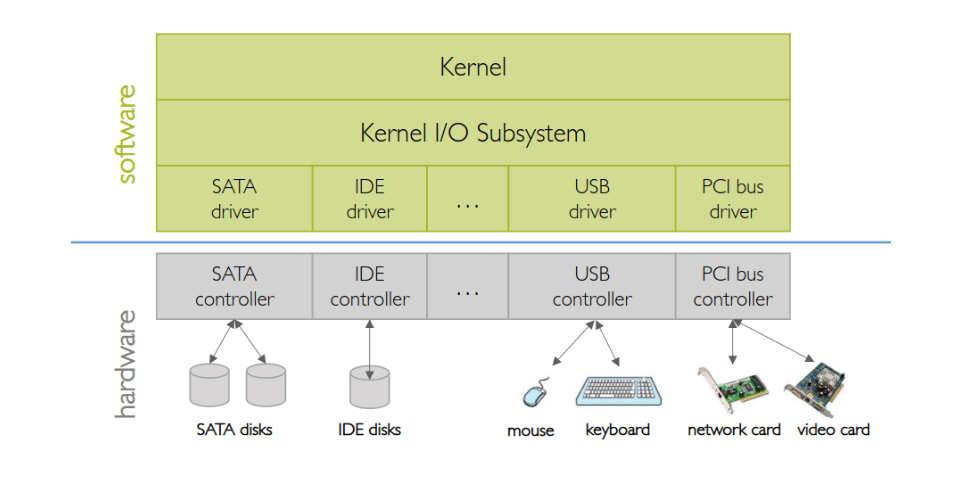
\includegraphics[width=0.6\textwidth,keepaspectratio]{{im/1_3}}
        \caption{Alcuni dei componenti di un semplice personal computer}    
    \end{center}
    \end{figure}

    \subsubsection{System Bus}
    Inizialmente veniva usato un unico bus per gestire tutto il traffico. Combina le funzioni di 
    \begin{itemize}
        \item Data bus effettivo di informazioni
        \item Address bus per determiare dove tali informazioni devono essere inviate
        \item Control bus per indicare quali operazioni dovrebbero essere eseguite
    \end{itemize}
    Sono stati aggiunti più bus dedicati per gestire il traffico da CPU a memoria e I/O, PCI, SATA, USB, ecc.
    
    \subsubsection{Dispostivi di I/O}
    Ogni dispositivo I/O è composto da due parti fondamentali il dispositivo fisico stesso e il controller del dispositivo (chip o set di chip che controllano una famiglia di dispositivi fisici).\\
    Il sistema operativo comunica con un controller del dispositivo utilizzando un driver di dispositivo specifico.\\
    La communicazione con i Dispositivi di Controllo ciacun controller del dispositivo ha un numero di registri dedicati per comunicare con esso:
    \begin{itemize}
        \item Registri di stato: forniscono alla CPU informazioni sullo stato del dispositivo I/O (ad esempio, inattivo, pronto per l'input, occupato, errore, transazione completata)
        \item Registri di configurazione/controllo utilizzati dalla CPU per configurare e controllare il dispositivo
        \item Registri dati utilizzati per leggere o inviare dati al dispositivo I/O
    \end{itemize}
    La CPU riesce ad indirizzare mettendo l'address di un byte di memoria nel address bus, specficando il segnale \texttt{READ} sul controllo del bus. Alla fine, la RAM risponderà con il contenuto della memoria sul Data bus.
    
    La CPU può comunicare con un controller del dispositivo in due modi:
    \begin{itemize}
        \item I/O mappati alle porte che fanno riferimento ai registri del controller utilizzando un I/O separato
        spazio degli indirizzi. \\Il registro di ciascun controller del dispositivo I/O è mappato su una porta specifica (indirizzo).\\
        Richiede classi speciali di istruzioni CPU (ad es. IN/OUT). L'istruzione \texttt{IN} legge da un dispositivo I/O, mentre \texttt{OUT} scrive. Quando si usano le istruzioni IN o OUT, l' \texttt{M/\#IO} non viene asserito, quindi la memoria non risponde e il chip I/O sì.
        \item I registri del controller del Memory-Mapped I/O utilizzano lo stesso spazio di indirizzamento utilizzato dalla memoria principale.\\Il Memory-mapped I/O "spreca" parte dello spazio degli indirizzi ma non necessita di istruzioni speciali. Per le porte del dispositivo I/O della CPU sono proprio come i normali indirizzi di memoria. La CPU utilizza istruzioni simili a \texttt{MOV} per accedere ai registri del dispositivo I/O. In questo modo viene asserito l' \texttt{M/\#IO} indicando l'indirizzo richiesto dalla CPU riferito alla memoria principale
    \end{itemize}
    Per eseguire le attività di I/O, vengono utilizzate due modalità di gestione:
    \begin{itemize}
        \item Polling
        \item La CPU periodicamente verifica lo stato dei task delle attività di I/O
        \item Interrupt-driven dove la CPU riceve un segnale di interrupt dal controller una volta che la task I/O viene completata
        \item La CPU riceve un interrupt dal controller (device o DMA \footnote{Direct Memory Access}) una volta finito il task dell'I/O (con successo o in modo anomalo)
        \item La CPU svolge il lavoro effettivo di spostamento dei dati
        \item La CPU delega il lavoro a un controller DMA dedicato
    \end{itemize}

\subsubsection{Processori}
La CPU preleva le istruzioni della memoria (esegue il \textbf{fetch}) e le esegue. La CPU si occupa poi si decodificarla per determinare il tipo e gli operandi , eseguirla e poi prelevare, decodificare ed eseguire le successive. Poichè accedere alla memoria richiede molte risorse tutte le CPU contengono all'interno dei \textbf{registri}  per memorizzare variabili importanti o risultati temporanei. Oltre ai registri i computer contengono il \textbf{program counter (PC)}, contente l'indirizzo di memoria in sui si trova la successiva istruzione da seguire, dopodichè viene il PC viene aggiornato per posizionarsi sulla successiva. \\
Un altro registro è lo \textbf{stack pointer} che punta alla cima dello stack attuale. Un altro registro è il \textbf{program status word (PSW)} che contiene i bit di condizione, impostati da istruzioni di confronto, la prorità della CPU, la modalità (kernel o utente) e altri bit di controllo. 
Nelle architetture più moderne, vengono implementati più livelli di protezione, detti protection rings. Ogni ring aggiunge restrizioni sulle istruzioni eseguibili dalla CPU.
\begin{figure}[hbt]
    \begin{center}
        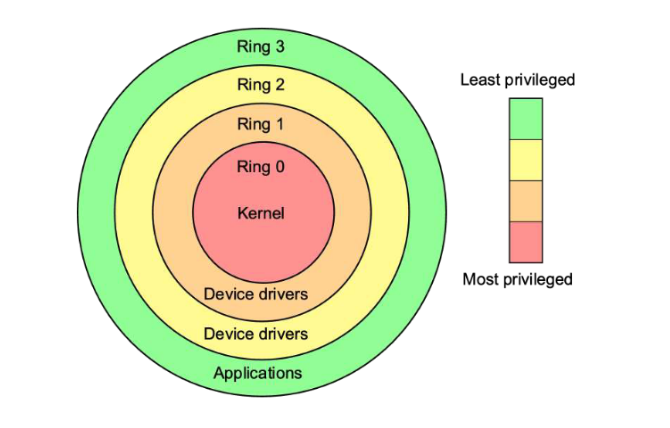
\includegraphics[width=0.5\textwidth,keepaspectratio]{{im/ring}}
        \caption{Protection Rings}    
    \end{center}
    \end{figure}

Un modo semplice per avere una protezione alla memoria è quello di avere due registri dedicati:
\begin{itemize}
    \item Base $\rightarrow$ contenente il primo address di partenza 
    \item Limite $\rightarrow$ contenente l'ultimo address valido 
\end{itemize}
Il sistema operativo carica i rigistri di base e limite all'avvio del programma mentre la CPU controlla che ogni indirizzo di memoria a cui fa riferimento il programma utente rientri tra i valori base e limite.


Per ottenere servizi dall'OS un programma utente deve fare una \textbf{system call (chiamata di sistema)} che entra nel kernel e richiama l'OS. Quando il lavoro è stato completato il controllo è restituito al programma utente.\\
L'istruzione \texttt{TRAP} cambia la modalità da utente a kernel e avvia l'OS. 
\begin{itemize}
    \item System call (software trap), ossia la richiesta di un servizio dell'OS, svolte in modo sincrono e innescate dai software
    \item Exception (fault), ossia la gestione di errori dovuti ad eventi inattesi, svolte in modo sincrono e innescate dai software
    \item Interrupt, ossia il completamento di una richiesta in attesa, svolte in modo asincrono e innescate dall'hardware
\end{itemize}

Esistono sei categorie importanti di System call:
\begin{itemize}
    \item \textbf{Process control} include \texttt{end}, texttt{abort}, texttt{load}, texttt{execute}, creazione e terminazione di processi, get/set attributi di processi, attesa, signal event, e allocazione di memoria libera. Quando un processo si interrompe o si interrompe, è necessario avviarne o riprenderne un altro. Quando i processi si arrestano in modo anomalo, potrebbe essere necessario fornire core dump e/o altri strumenti diagnostici o di ripristino
    \item \textbf{File management} crea file, elimina file, apri, chiudi, leggi, scrivi, riposiziona, ottieni attributi di file e imposta attributi di file. Queste operazioni possono essere supportate anche per directory e file ordinari. L'effettiva struttura della directory può essere implementata utilizzando file ordinari sul file system o tramite altri mezzi (ne parleremo più avanti)
    \item \textbf{Device management} include dispositivi di richiesta, dispositivi di rilascio, lettura, scrittura, riposizionamento, recupero/impostazione degli attributi del dispositivo e collegamento o scollegamento logico dei dispositivi. I dispositivi possono essere fisici (ad es. unità disco) o virtuali/astratti (ad es. file, partizioni e dischi RAM). Alcuni sistemi rappresentano i dispositivi come file speciali nel file system, in modo che l'accesso al "file" richieda il driver di dispositivo del sistema operativo appropriato. E.g la directory \texttt{/dev} su qualsiasi sistema \texttt{UNIX}
    \item \textbf{Information maintenance} nclude le chiamate per ottenere/impostare l'ora, la data, i dati di sistema e gli attributi di processo, file o dispositivo. I sistemi possono anche fornire la possibilità di eseguire il dump della memoria in qualsiasi momento. Programmi a passo singolo che interrompono l'esecuzione dopo ogni istruzione e tracciano
    il funzionamento dei programmi (debug) 
    \item \textbf{Communications} include creazione/eliminazione di connessioni di comunicazione, invio/ricezione di messaggi, trasferimento di informazioni sullo stato e collegamento/scollegamento di dispositivi remoti. Esisono due modelli di comunicazione: 
    \begin{itemize}
        \item scambio di messaggi: il modello di trasmissione dei messaggi deve supportare le chiamate a:
        \begin{itemize}
            \item Identificare un processo remoto e/o un host con cui comunicare
            \item Stabilire una connessione tra i due processi
            \item Aprire e chiudere la connessione secondo necessità
            \item Trasmettere messaggi lungo la connessione
            \item Attendere i messaggi in arrivo, in stato di blocco o non blocco
            \item Eliminare la connessione quando non è più necessaria
            
            Più semplice e facile (in particolare per le comunicazioni tra computer) e generalmente appropriato per piccole quantità di dati
        \end{itemize}
        \item memoria condivisa: il modello di memoria condivisa deve supportare le chiamate a:
        \begin{itemize}
            \item  Creare e accedere alla memoria condivisa tra processi (e thread) 
            \item Fornire meccanismi di blocco che limitano l'accesso simultaneo
            \item Liberare memoria condivisa e/o allocarla dinamicamente secondo necessità
            
            Più veloce e generalmente l'approccio migliore in cui devono essere condivise grandi quantità di dati
            Ideale quando la maggior parte dei processi deve leggere i dati anziché scriverli
        \end{itemize}
    \end{itemize}
\end{itemize}

\subsubsection{Protezione delle system call}
Fornisce meccanismi per controllare quali utenti/processi hanno accesso a quali risorse di sistema. Le chiamate di sistema consentono di regolare i meccanismi di accesso secondo necessità. Agli utenti non privilegiati può essere concesso temporaneamente un accesso elevato autorizzazioni in circostanze specifiche. 
Quando un programma utente richiede l'esecuzione di una syscall tramite un'API fornita dal sistema operativo, tale richiesta viene prima convertita in linguaggio macchina, per poi venir gestita da \textbf{System call Handler}, il quale si occuperà di salvare lo stato precedente dei registri, i quali verranno poi alterati durante l'esecuzione della syscall, per poi essere ripristinati. 

\subsubsection{Passaggio di parametri}
Esistono 3 metodi usati per passare parametri :
\begin{itemize}
    \item Salvare i parametri in registri
    \item Salvare parametri in \texttt{block} o \texttt{table} di un'area di memoria dedicata
    \item Parametri inseriti nello stack dal programma e estratti dallo stack dal sistema operativo (più complessi a causa dei diversi spazi degli indirizzi!)
\end{itemize}
I metodi block e stack non limitano il numero o la lunghezza dei parametri passati
\begin{figure}[hbt]
    \begin{center}
        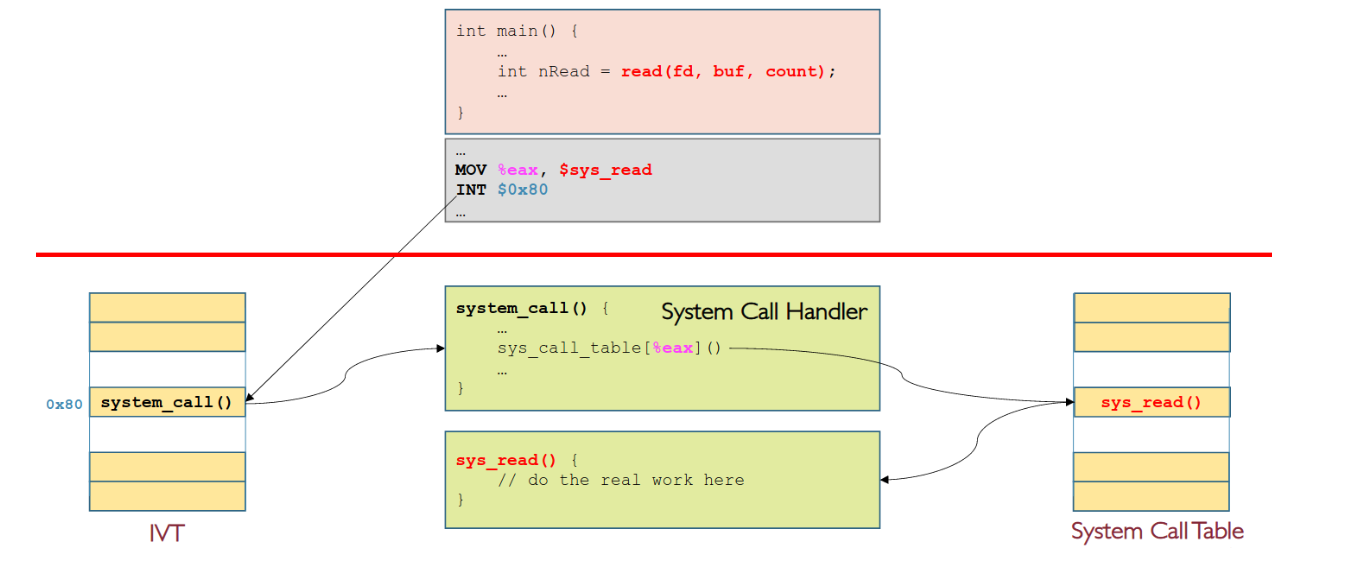
\includegraphics[width=0.9\textwidth,keepaspectratio]{{im/ivt}}
        \caption{System call Handler}    
    \end{center}
    \end{figure}
\subsubsection{Timer, Istruzioni atomiche, Virtual Memory}
Il timer è una funzionalità hardware per abilitare la pianificazione della CPU. Nei sistemi multi-tasking, permette alla CPU di non essere monopolizzata da processi "egoistici". Il timer genera un interrupt e ad ogni sua interruzione, lo scheduler della CPU prende il sopravvento e decide quale processo da eseguire successivamente.\\
Gli interrupt possono verificarsi in qualsiasi momento e interferire con i processi in esecuzione e l'OS deve essere in grado di sincronizzare le attività di cooperazione, simultanee processi, garantire che brevi sequenze di istruzioni (ad es. lettura-modifica-scrittura) vengano eseguite atomicamente da disabilitare gli interrupt prima della sequenza e riabilitarli successivamente o istruzioni speciali che vengono eseguite nativamente in modo atomico. \\
La virtualizzazionde della memoria è un'astrazione (dell'effettiva memoria principale fisica), conferisce ad ogni processo l'illusione che la memoria fisica sia solo contigua spazio degli indirizzi (spazio degli indirizzi virtuali). Permette di eseguire programmi senza che vengano caricati interamente nella memoria principale. Può essere implementata sia in HW (MMU) che in SW (OS).
\begin{itemize}
    \item MMU Associa gli indirizzi virtuali a quelli fisici tramite una tabella delle pagine gestita dal sistema operativo. Utilizza una cache denominata Translation Look-aside Buffer (TLB) con "mappature recenti" per ricerche più rapide. Il sistema operativo deve sapere quali pagine sono caricate nella memoria principale e quali su disco
    \item Il sistema operativo è responsabile della gestione degli spazi di indirizzi virtuali
\end{itemize}


\begin{figure}[hbt]
    \begin{center}
        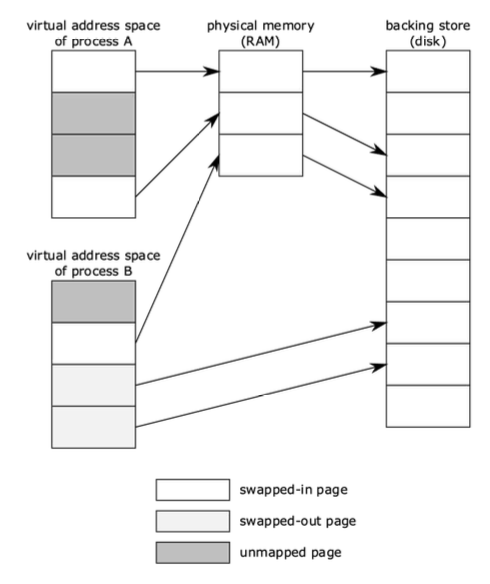
\includegraphics[width=0.3\textwidth,keepaspectratio]{{im/virtualm}}
        \caption{Virtual vs. Physical Address Space}    
    \end{center}
    \end{figure}

Lo spazio degli indirizzi virtuali è tipicamente suddiviso in blocchi contigui della stessa dimensione (ad esempio, 4 KiB), chiamati pagine (\textbf{pages}). Ciascuna pagina che non sono caricate nella memoria principale vengono memorizzate su disco.

\pagebreak

\subsection{Progettazione e implementazione del sistema operativo}
La struttura interna dei diversi sistemi operativi può variare notevolmente e gli obiettivi del sistema è facilare l'usabilità rispetto al progettare/implementare. È fondamentale separare le politiche dai meccanismi della policy ovvero \textit{cosa} sarà fatto e il meccanismo che indica \textit{come} farlo.
Il disaccoppiamento della logica della politica dal meccanismo sottostante è un principio di progettazione generale nell'informatica, in quanto migliora il sistema:
\begin{itemize}
    \item flessibilità: l'aggiunta e la modifica delle politiche possono essere facilmente supportate
    \item riusabilità: i meccanismi esistenti possono essere riutilizzati per implementare nuove politiche 
    \item stabilità: l'aggiunta di una nuova politica non destabilizza necessariamente il sistema    
\end{itemize}
Le modifiche ai criteri possono essere facilmente regolate senza riscrivere il codice.

I primi sistemi operativi sviluppati in linguaggio assembly, e uno dei vantaggi era il controllo diretto sull'HW (alta efficienza) mentre uno svantaggio può essere il legame con uno specifico HW (bassa portabilità). Oggi, un misto di lingue infatti i livelli più bassi in assembly il corpo principale in C e i programmi di sistema in C, C++, linguaggi di scripting come PERL, Python, ecc.
Il sistema operativo dovrebbe essere suddiviso in sottosistemi separati, ciascuno con compiti, input/output e caratteristiche prestazionali accuratamente definiti. Esistono vari modi di strutturare un sistema operativo: 

\begin{itemize}
    \item \textbf{Struttura semplice} $\rightarrow$ MS-DOS, dove non vi è alcun sottosistema e non vi è separazione tra kernel e user mode (esempio: il sistema MS-DOS). Semplice da implementare ma estremamente insicuro e poco rigido.
    \item  \textbf{Struttura a Kernel Monolitico} $\rightarrow$ UNIX, dove l'intero sistema operativo opera in kernel mode e solo i software utente lavorano in user mode (esempio: il sistema UNIX). Semplice da implementare ed efficiente, ma ancora poco sicuro e rigido
    \item \textbf{Struttura a livelli} $\rightarrow$, MULTICS dove l'OS è suddiviso in N livelli ed ogni livello L usa funzio- nalità implementate dal livello L1 ed espone nuove funzionalità al livello L + 1. Per via della struttura a livelli, il sistema è molto modulare, portabile e semplice da debuggare, rendendo tuttavia più complessa per la comunicazione tra di essi.
    \item \textbf{Struttura a Microkernel}, dove il kernel contiene solo le funzionalità di base, men- tre tutte le altre funzionalità dell'OS e i programmi utente vengono eseguiti in user mode. Tale struttura porta ad una maggiore sicurezza, affidabilità ed estensibilità, ma anche ad un'efficienza ridotta.
    \item \textbf{Struttura a Moduli del Kernel caricabili (LKM)}, dove l'OS utilizza dei moduli tramite cui accedere alle funzionalità del kernel
    \item \textbf{Sistema a Kernel Ibrido}, dove viene utilizzato un approccio intermedio al kernel monolitico e al microkernel, ottenendo i vantaggi di entrambi gli approcci
\end{itemize}
\pagebreak
%-------------------------------------------------------%
\section{Gestione dei Processi e thread}

Un programma è un file eseguibile che risiede nella memoria persistente (ad es. disco) e contiene solo l'insieme di istruzioni necessarie per eseguire un lavoro specifico. Un processo è l'astrazione del sistema operativo di un programma in esecuzione (unità di esecuzione). Il processo è dinamico, mentre un programma è statico (solo codice e dati). Diversi processi possono eseguire lo stesso programma (ad esempio, multiple istanze di Google Chrome) ma ognuna ha il proprio stato. Un processo esegue un'istruzione alla volta, in sequenza. \\

Il sistema operativo fornisce la stessa quantità di spazio di indirizzi virtuali a ciascun processo. Lo spazio degli indirizzi virtuali è un'astrazione dello spazio degli indirizzi della memoria fisica. L'intervallo di indirizzi virtuali validi che un processo può generare dipende dalla macchina. Avremo perciò:
\begin{itemize}
    \item \textbf{Text} contenente le istruzioni dell'eseguibile
    \item \textbf{Data} Variabili globali e statiche inizializzate
    \item \textbf{BSS} variabile globale e statica (non inizializzata o inizializzata a 0)
    \item \textbf{Stack} Struttura LIFO utilizzata per memorizzare tutti i dati necessari a una chiamata di funzione (stack frame)
    \item \textbf{Heap} usata per l'allocazione dinamica
\end{itemize}

\begin{figure}[hbt]
    \begin{center}
        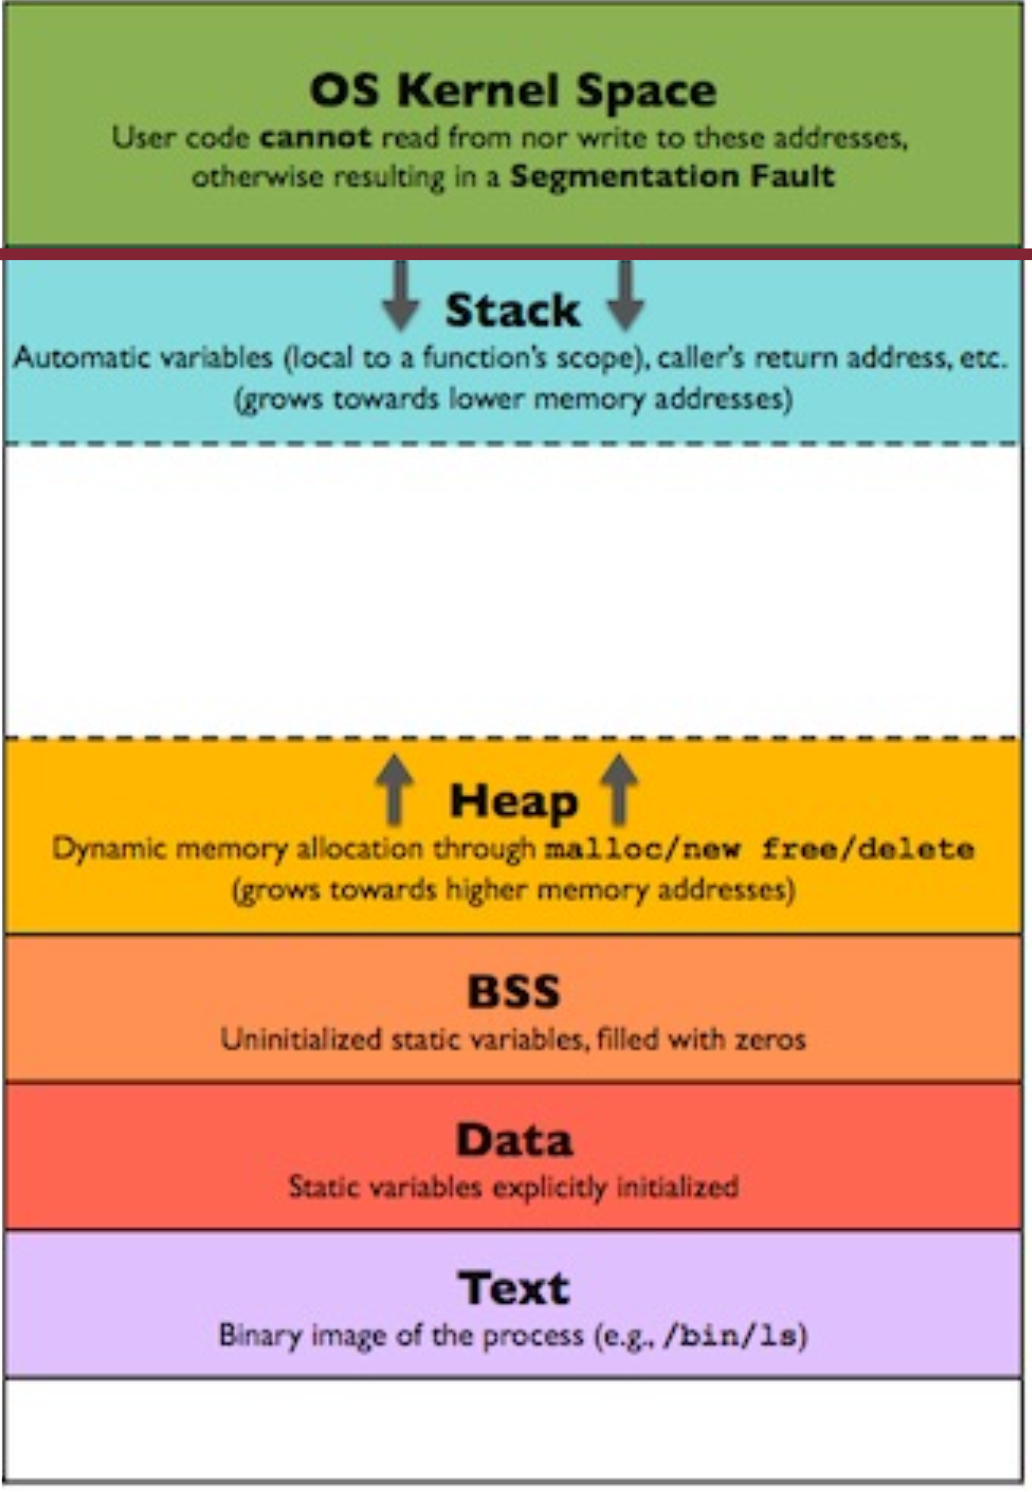
\includegraphics[width=0.3\textwidth,keepaspectratio]{{im/virtualaddress}}
        \caption{Virtual Address Space Layout}    
    \end{center}
    \end{figure}

Sullo stack sono definite due operazioni: \textbf{push} e \textbf{pop}. Il push viene usato per inserire degli elementi, mentre pop per rimuoverli. Usa un registro dedicato (e.g \texttt{esp}) il cui contenuto è l'indirizzo nella memoria principale della parte superiore dello stack. La memoria dello stack cresce convenzionalmente dall'alto verso il basso, cioè dagli indirizzi di memoria più alti a quelli più bassi. Ogni funzione utilizza una porzione dello stack, chiamata stack \textbf{frame} e in ogni momento possono esistere contemporaneamente più stack frame, a causa di diverse chiamate di funzioni nidificate, ma solo una è attiva.
Lo stack frame per ogni funzione è diviso in tre parti:
\begin{itemize}
    \item parametri della funzione + indirizzo di ritorno
    \item back-pointer allo stack frame precedente
    \item variabili locali
\end{itemize}
Il primo è impostato dal chiamante, il secondo e il terzo vengono impostati dal chiamato. Il puntatore \texttt{esp} viene sempre aggiornato man mano che lo stack cresce ed è difficile per il chiamato accedere ai parametri effettivi senza un riferimento fisso nello stack. Per risolvere questo problema invece di utilizzare un singolo puntatore in cima allo stack usa un puntatore aggiuntivo alla parte inferiore (base) dello stack (\texttt{ebp}) lascia che \texttt{esp} sia libero di cambiare tra diverse chiamate di funzione, mentre tiene \texttt{ebp} fissato all'interno di ogni stack frame. \\

\begin{figure}[hbt]
    \begin{center}
        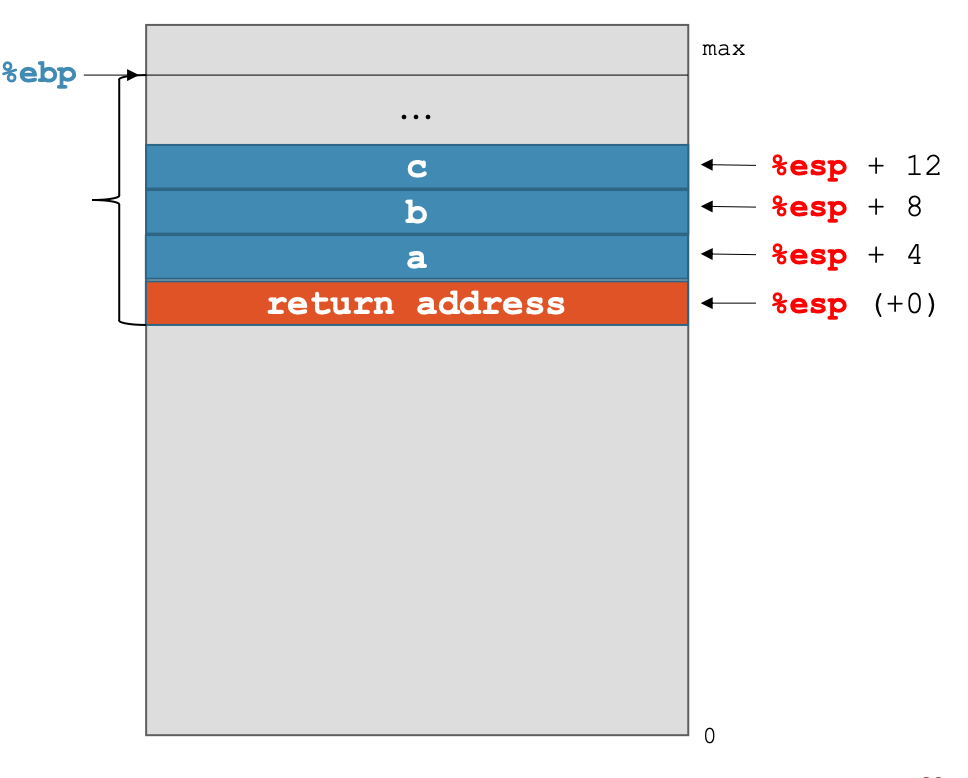
\includegraphics[width=0.5\textwidth,keepaspectratio]{{im/ebp}}
        \caption{Function Parameters + Return}    
    \end{center}
    \end{figure}
\subsection{Stato di esecuzione del processo}
In ogni momento un processo può trovarsi in uno dei seguenti cinque stati:
\begin{itemize}
    \item \textbf{Ready}, il processo è pronto per essere eseguito ma attende di essere programmato sulla CPU
    \item \textbf{Running}, il processo sta effettivamente eseguendo istruzioni sulla CPU 
    \item \textbf{Waiting}, il processo è sospeso in attesa che una risorsa sia disponibile o un
    evento da completare/verificare (ad es. input da tastiera, accesso al disco, timer, ecc.)
    \item \textbf{Terminated}, il processo è terminato e il sistema operativo può distruggerlo
\end{itemize}

\begin{figure}[hbt]
    \begin{center}
        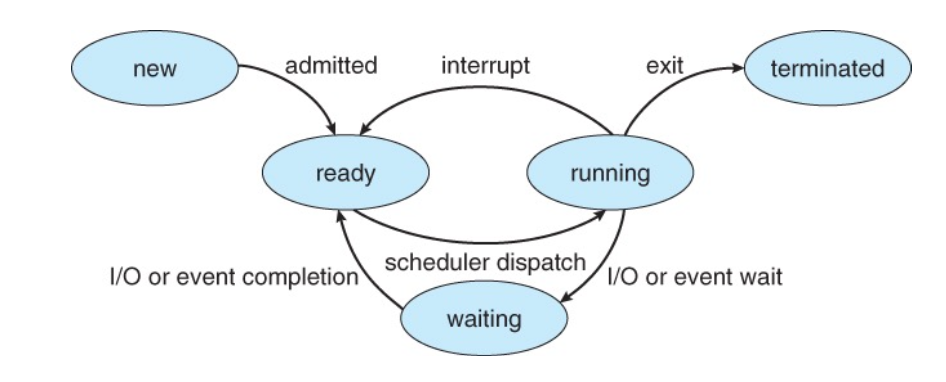
\includegraphics[width=0.7\textwidth,keepaspectratio]{{im/diagramma}}
        \caption{Process Execution State Diagram}    
    \end{center}
    \end{figure}

Durante l'esecuzione, il processo passa da uno stato all'altro in base alle azioni del programma (ad esempio, chiamate di sistema) come azioni del sistema operativo (ad es. pianificazione) o azioni esterne (ad es. interruzioni).\\ 

La maggior parte delle chiamate di sistema (ad esempio quelle di I/O) sono bloccanti. Il processo chiamante (spazio utente) non può fare nulla fino al ritorno della chiamata di sistema. Il sistema operativo (spazio del kernel) si occupa di:
\begin{itemize}
    \item impostare il processo corrente in uno stato di attesa (ovvero, in attesa del ritorno della chiamata di sistema)
    \item  pianifica un diverso processo pronto per evitare che la CPU sia inattiva
\end{itemize} 
Una volta che la chiamata di sistema ritorna, il processo precedentemente bloccato è pronto per essere schedulato nuovamente per l'esecuzione.
\footnote{NOTA: l'intero sistema non è bloccato, solo il processo che ha richiesto la chiamata bloccata è!}\\
Lo stato del processo è costituito da: 
\begin{itemize}
    \item il codice del programma in esecuzione
    \item i dati statici del programma in esecuzione
    \item il program counter (PC) che indica la prossima istruzione da eseguire
    \item Registri CPU
    \item la catena di chiamate del programma (stack) insieme ai puntatori di frame e stack
    \item lo spazio per l'allocazione dinamica della memoria (heap) insieme al \item puntatore heap l'insieme di risorse in uso (ad es. file aperti)
    \item lo stato di esecuzione del processo (pronto, in esecuzione, ecc.)
\end{itemize}

\subsection{Process Control Block (PCB)}
Il \textbf{PCB} è la struttura dati principale utilizzata dal sistema operativo per tenere traccia di qualsiasi processo. Il PCB tiene traccia dello stato di esecuzione e della posizione di un processo. Il sistema operativo assegna un nuovo PCB alla creazione di un processo e lo inserisce in una coda di stato e viene deallocato non appena termina il processo associato. \\
Il PCB contiene:
\begin{itemize}
    \item Stato del processo pronto, in attesa, in esecuzione, ecc.
    \item Numero di processo (ovvero identificatore univoco)
    \item Program Counter (PC) + Stack Pointer (SP) + registri di uso generale 
    \item Informazioni sulla pianificazione della CPU priorità e puntatori alle code di stato 
    \item Informazioni sulla gestione della memoria tabelle delle pagine
    \item Informazioni sull'account à tempo utilizzato dalla CPU del kernel e dell'utente, stato I/O del proprietario 
    \item Elenco dei file aperti
\end{itemize}
\begin{figure}[hbt]
    \begin{center}
        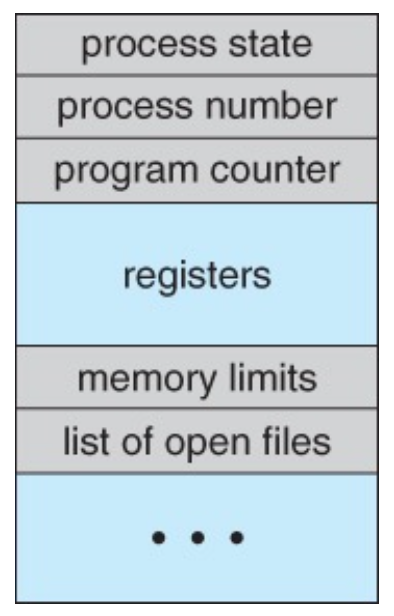
\includegraphics[width=0.2\textwidth,keepaspectratio]{{im/PCB}}
        \caption{Process Execution State Diagram}    
    \end{center}
    \end{figure}

\subsection{Creazione di processi}
I processi possono creare altri processi tramite specifiche chiamate di sistema. Il processo creatore è chiamato genitore del nuovo processo, chiamato figlio. Il genitore condivide risorse e privilegi con i suoi figli. Un genitore può aspettare che un figlio finisca o continuare in parallelo.\\
A ogni processo viene assegnato un identificatore intero (noto anche come identificatore di processo o PID) e per ogni processo viene memorizzato anche il PID genitore (PPID).\\
Sui tipici sistemi UNIX lo scheduler del processo è denominato \texttt{sched} e riceve il PID 0. La prima cosa che fa all'avvio del sistema è lanciare \texttt{init}, che dà a quel processo il PID 1. Successivamente \texttt{init} avvia tutti i daemons di sistema e i login degli utent,i e diventa il genitore ultimo di tutti gli altri processi. I processi vengono creati attraverso la chiamata di sistema \texttt{fork()}.

\begin{figure}[hbt]
    \begin{center}
        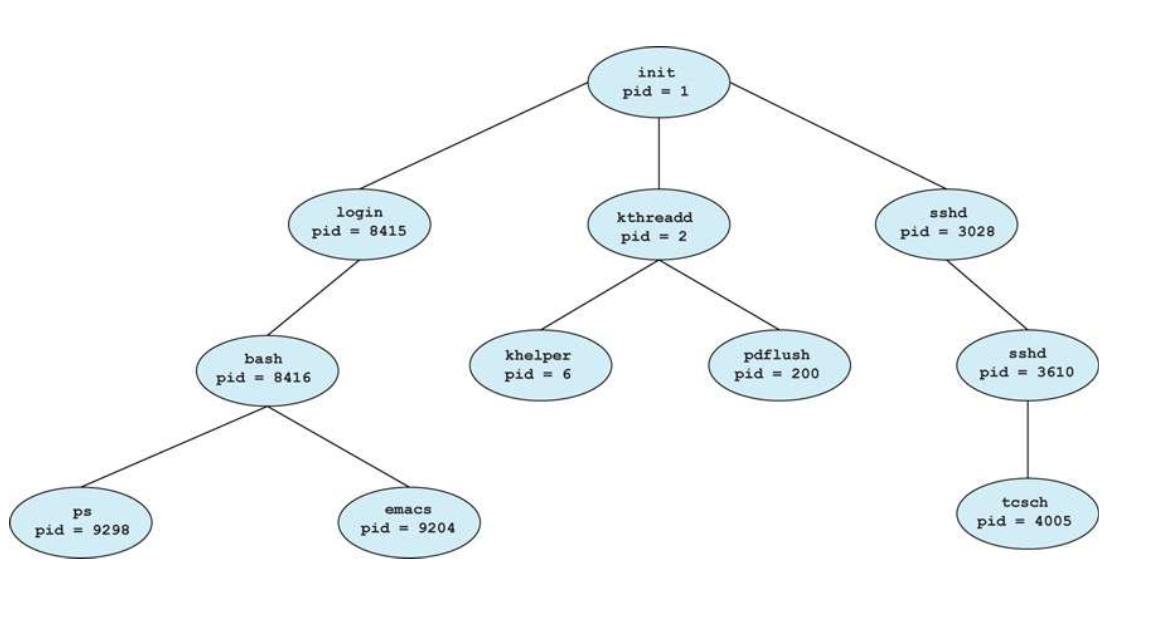
\includegraphics[width=0.7\textwidth,keepaspectratio]{{im/creazioneProcessi}}
        \caption{Process Creation: UNIX/Linux}    
    \end{center}
    \end{figure}
\subsubsection*{Creazione del processo: risorse del padre vs figlio}
Abbiamo due possibilità per lo spazio degli indirizzi del figlio rispetto al genitore:
\begin{itemize}
    \item Il bambino può essere un duplicato esatto del genitore, condividendo lo stesso programma e gli stessi segmenti di dati in memoria
    \item Ciascuno avrà il proprio PCB, inclusi program counter, registri e PID 
    \item Questo è il comportamento della chiamata di sistema fork in UNIX
    \item Il processo figlio può avere un nuovo programma caricato nel suo spazio degli indirizzi, con tutti i nuovi segmenti di codice e dati
    \item Questo è il comportamento delle chiamate di sistema di spawn in Windows
    \item I sistemi UNIX implementano ciò come secondo passaggio, utilizzando la chiamata di sistema exec
\end{itemize}
    
\subsection{Terminazione di processi}

\subsection{Scheduling dei processi}
\subsection{Communicazione dei processi}




%-------------------------------------------------------%
\pagebreak

\section{Sincronizzazione tra Processi/Thread}
%-------------------------------------------------------%
\pagebreak

\section{Gestione della Memoria}
%-------------------------------------------------------%
\pagebreak

\section{Gestione dei Sistemi di I/O}
%-------------------------------------------------------%
\pagebreak

\section{File System}
%-------------------------------------------------------%
\pagebreak

\section{Advanced Topics}



\end{document}

